\documentclass[11pt]{article}
\usepackage{amsmath, amsfonts, amsthm, amssymb}  % Some math symbols
\usepackage{enumerate}
\usepackage{fullpage}
\usepackage{color}
\usepackage[x11names, rgb]{xcolor}
\usepackage{tikz}
\usepackage{graphicx}
\usepackage{listings}
\usepackage{fancyhdr}

% \usepackage{fontspec}
% \setmainfont{Times New Roman}

\renewcommand*{\familydefault}{\sfdefault}

\setlength{\parindent}{0pt}
\setlength{\parskip}{6pt}
\pagestyle{empty}

\pagestyle{fancy}
\fancypagestyle{firststyle}
{
   \lhead{\myname \\ \myandrew \\ \today \\ \vspace*{-.4em}}
   \rhead{15-221 \\ Fall 2014 \\ Section A \\ \vspace*{-.4em}}
   \setlength{\headsep}{45pt}
}

\newcommand{\myname}{Your name here}
\newcommand{\myandrew}{andrewid@andrew.cmu.edu}
\newcommand{\mytitle}{Project Proposal}
\title{Explainshell Chrome Extension \\ \vspace*{.5em} \Large\mytitle}
\date{}
%%%%%%%%%%%%%%%%%%%%%%%%%%%%%%%%%%%%%%%%%%%%%%%%%%%%%%%%%%%

\begin{document}
\pagenumbering{gobble} 
\clearpage\maketitle
\thispagestyle{firststyle}
\newpage
\pagenumbering{arabic}  
\lhead{\myname}
\rhead{\thepage}
\setlength{\voffset}{-50pt}
\setlength{\headsep}{25pt}

\section{Plan}

Our goal is to develop a Chrome extension that helps users learn the usage of shell commands found online and avoid malicious shell commands. After the user installs the extension from the Chrome extension store, it will scan any web page that the user visits for shell commands in the background, and allow users to simply hover / click on unfamiliar shell commands to view a detailed explanation of the shell commands in a pop-up window. This extension will not only help users learn and familiarize with the usage of nearly 30,000 shell commands, but will also help users identify potentially destructive or malicious commands before executing them. 

We will also create a back-end server to store and provide interesting analytics about trending shell commands, trending referring sites and other statistics. If time allows, we will also attempt to develop a more advanced web page parsing technique to identify shell commands in a web page, possibly using machine learning.

For this project, we have set up a Git repository that allows us to coordinate and keep track of code changes easily. We have also set up a Google Drive to keep track of our progress. We will set up team meetings at the end of each phase by email or texting.

\section{Benefits}

This project will benefit both our team and end users. For users, the project will provide a convenient way to look up and learn the usage of unfamiliar shell commands found online. Considering that shell commands are often powerful and can sometimes be malicious, the project can also potentially automatically warn users about malicious shell commands before they execute the commands. 

We will learn to use and familiarize with a lot of technologies in the process as well, including Git, Chrome extension, Javascript and Python. Through the process, we will also contribute to the explainshell open source project.

\section{Approach}
\subsection{Methodology}

In this section, we will explain the various technologies that we we will be using to complete the project. Through our project, we will develop a Chrome extension and a back-end server that provides analytics about trending shell commands. We will also contribute to the current code base of the open source explainshell project. 

For the Chrome extension, we will use Javascript and jQuery to scan and parse the webpage that user visits, to identify potential shell commands within a web page. We will then use AJAX to send requests to the explainshell API and receive documentations of identified commands. We will also use HTTP + CSS to layout a pop-up window that displays the documentation. 

We will also create a back-end server with [Python Flask (or Django?)]. The back-end server will store the history of shell commands that users look up using our extension, using a SQL database. The data will allow us to provide analytics and visualization about popular or trending searches.

\subsection{Project Schedule}
Specifically, our project will be separated into the following four phases. 

\par{\bf Phase 1}\\ 
We will first build a simple Chrome extension that allows user to look up the usage of shell command by highlighting any text in the browser window. Upon highlighting, a button will appear next to the highlighted text region. The user may click the button, which will instantly redirect the user to the corresponding usage documentation at the explainshell website in a new browser tab.

\par{\bf Phase 2}\\
We will refine our Chrome extension developed in Phase 1. Instead of asking the user to highlight the shell command that they want to look up, the Chrome extension will now automatically parse and search the web page to identify any shell commands. Upon identifying potential commands, the extension will turn the command into a clickable link, which will redirect the user to the usage documentation at the explainshell website.

\par{\bf Phase 3}\\
We will contribute to the code base of the explainshell project by adding an HTTP API, since this would also help us further improve our chrome extension. With the API, the Chrome extension may now display a pop-up window in the page, whenever the user hovers / clicks on the identified shell commands, whereas previously we always redirect the user to the documentation web page.

\par{\bf Phase 4}\\
We will develop a back-end server that provides analytics that allow users to view trending searches and referral sites. [Insert more description here]

Please refer to Fig. \ref{fig:timetable} on page \pageref{fig:timetable} for a Gantt chart of our project schedule.

\section{Qualifications}
\par{\bf Justin Gallagher} 
\begin{itemize}
	\item Summer internship at Microsoft working on ASP.NET web applications using SQL databases
	\item Wrote backend for fully-featured webapps such as Gitorial and CMUEats
	\item 2 years of HTML/CSS/Javascript experience
\end{itemize}

\begin{figure}[htb]
\centering
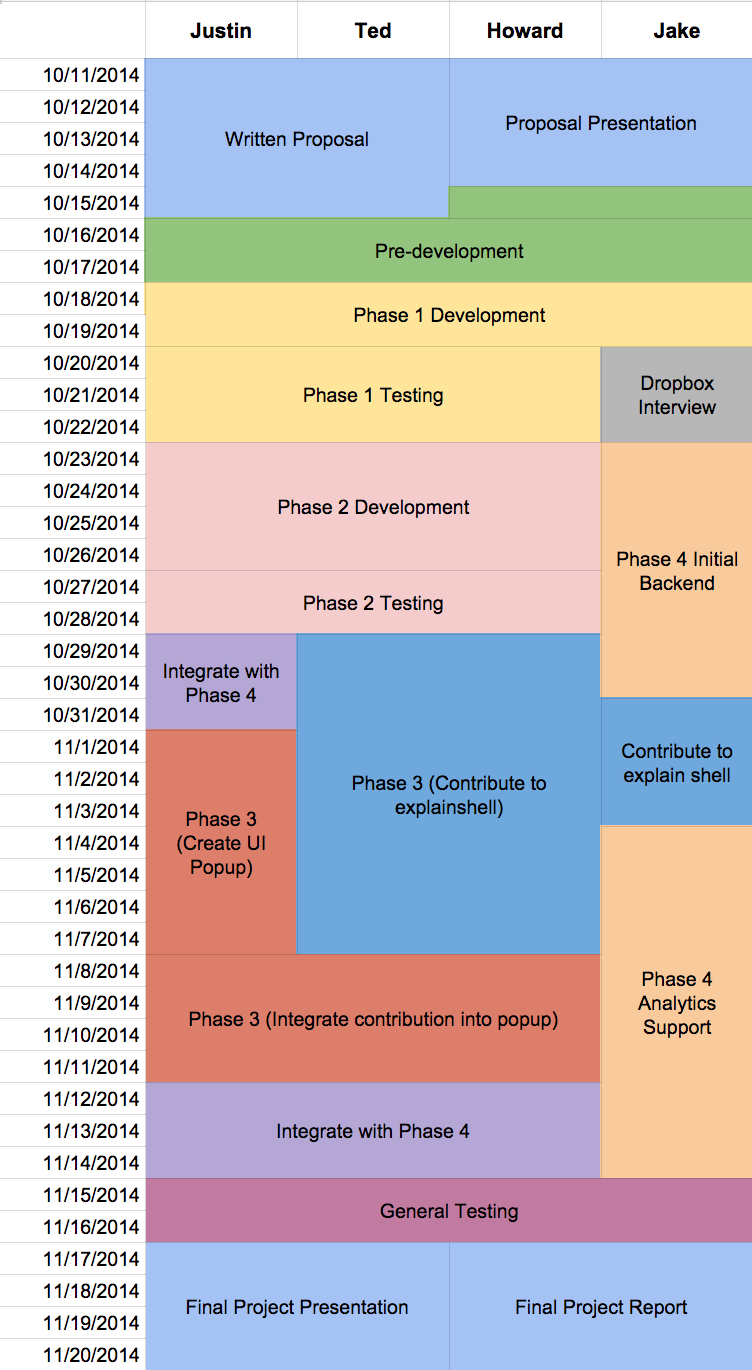
\includegraphics[width=.6\textwidth]{chart.png}
\caption{Project time line [To be converted into Gantt chart?]\label{fig:timetable}}
\end{figure}

\end{document}
